\documentclass[a4paper]{article}

% for dvipdfm:
%\def\pgfsysdriver{pgfsys-dvipdfm.def}
\usepackage{pgfplots}
\pgfplotsset{compat=1.3}% <-- moves axis labels near ticklabels (respects tick label widths)

\begin{document}
\begin{figure}
	\centering
	\begin{tikzpicture}
	\begin{loglogaxis}
		\addplot coordinates {
			(1,1)
			(16,16)
			(32,64)
		};
	\end{loglogaxis}
	\end{tikzpicture}
	\caption{A small example}
\end{figure}

\begin{figure}
	\centering
	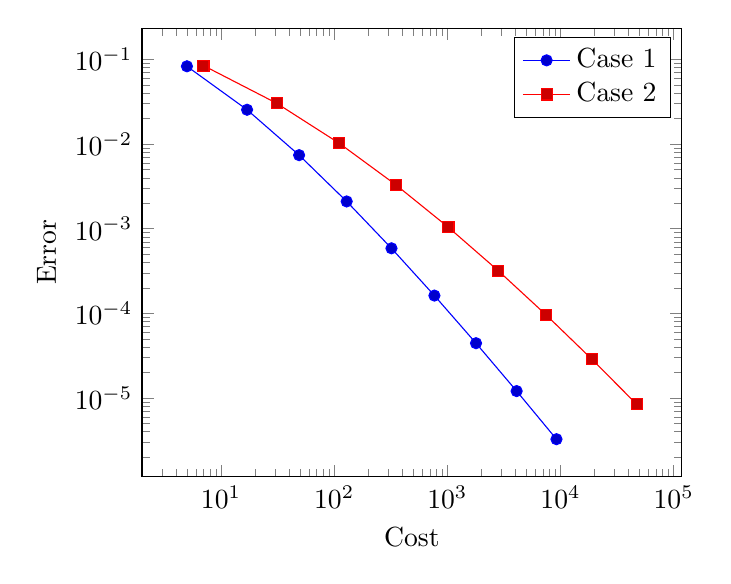
\begin{tikzpicture}
		\begin{loglogaxis}[
			xlabel=Cost,
			ylabel=Error]
		\addplot coordinates {
			(5,     8.31160034e-02)
			(17,    2.54685628e-02)
			(49,    7.40715288e-03)
			(129,   2.10192154e-03)
			(321,   5.87352989e-04)
			(769,   1.62269942e-04)
			(1793, 4.44248889e-05)
			(4097, 1.20714122e-05)
			(9217, 3.26101452e-06)
		};
		\addplot coordinates {
			(7,     8.47178381e-02)
			(31,    3.04409349e-02)
			(111,   1.02214539e-02)
			(351,   3.30346265e-03)
			(1023,  1.03886535e-03)
			(2815,  3.19646457e-04)
			(7423,  9.65789766e-05)
			(18943, 2.87339125e-05)
			(47103, 8.43749881e-06)
		};
		\legend{Case 1,Case 2}
		\end{loglogaxis}
	\end{tikzpicture}
	\caption{A larger example}
\end{figure}

\end{document}
